\newpage
\appendix

\section{Anhang 1}

\begin{table}[h]
  \begin{tabular}{lll}
    \toprule
    Kategorie & Eigenschaft\\
    \midrule
    \multirow[t]{2}{*}{Languages/Buildpacks (SAP supported)} & Node.js  \\
     & Java \\
     \multirow[t]{5}{*}{Languages/Buildpacks (Community supported)} & Python \\
     & PHP \\
     & Ruby \\
     & .NET Core \\
     & viele weitere \\
     \multirow[t]{6}{*}{Storage/Messaging Services} & SAP HANA, inkl. XSA Applications \\
     & MongoDB \\
     & PostgreSQL \\
     & Redis \\
     & RabbitMQ \\
     & Object Store, Unstructured Storage \\
     \multirow[t]{3}{*}{Integrated SSO Secrurity Cloud Connector} & Services für Authentifizierung,\\
     & Single Sign-on \\
     & und On-Premise Integrtion \\
     \multirow[t]{3}{*}{Integrated SSO Secrurity Cloud Connector} & AWS - EU, US East\\
     & Azure - US West  \\
    \bottomrule
    \end{tabular}
    \label{cf_table}
  \caption[Eigenschaften der Cloud-Foundry-Umgebung]{Eigenschaften der Cloud-Foundry-Umgebung \citep[S. 195]{Utecht2018}}
\end{table}

\section{Anhang 2}

\begin{figure}[h]
  \centering
  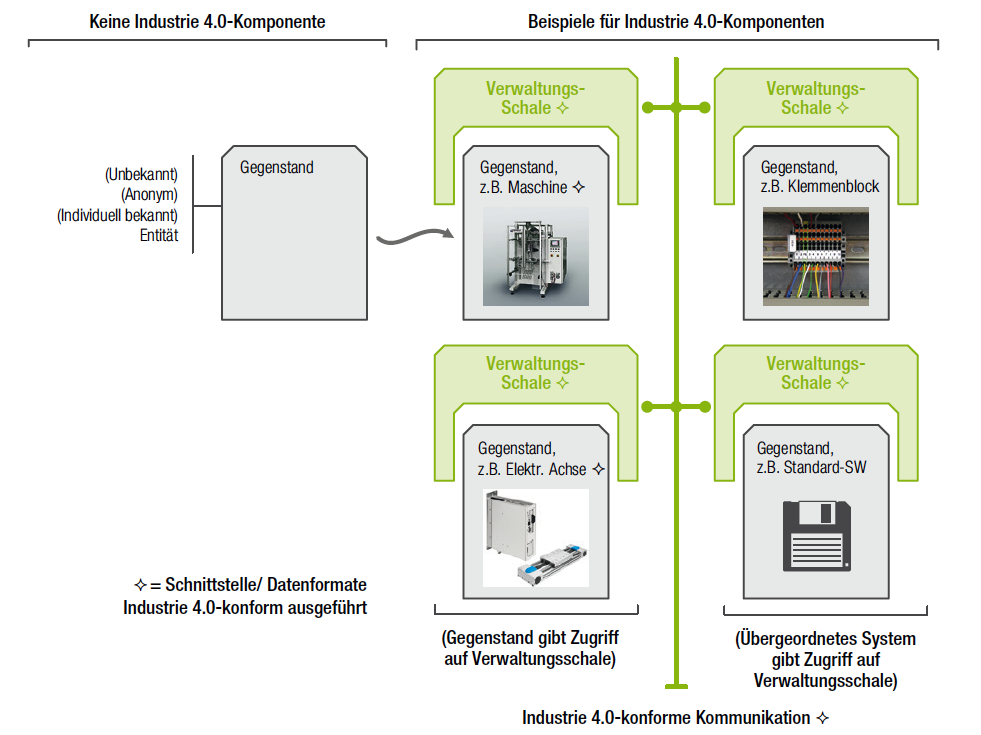
\includegraphics[width=1.1\linewidth]{Bsp_I40_Kompo.png}
  \caption[Beispiele für Industrie-4.0-Komponenten]{Beispiele für Industrie-4.0-Komponenten \citep[S. 54]{BITKOM2015}}
  \label{i40kompo}
\end{figure}

\begin{figure}[h]
  \centering
  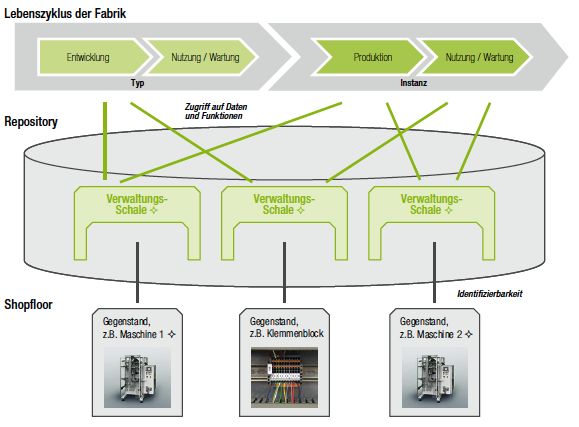
\includegraphics[width=1.1\linewidth]{I40_Lebenszyklus.png}
  \caption[Industrie-4.0-Komponenten im Lebensyklus der Fabrik]{Industrie-4.0-Komponenten im Lebensyklus der Fabrik \citep[S. 56]{BITKOM2015}}
  \label{lifecycle}
\end{figure}

\begin{figure}[h]
  \centering
  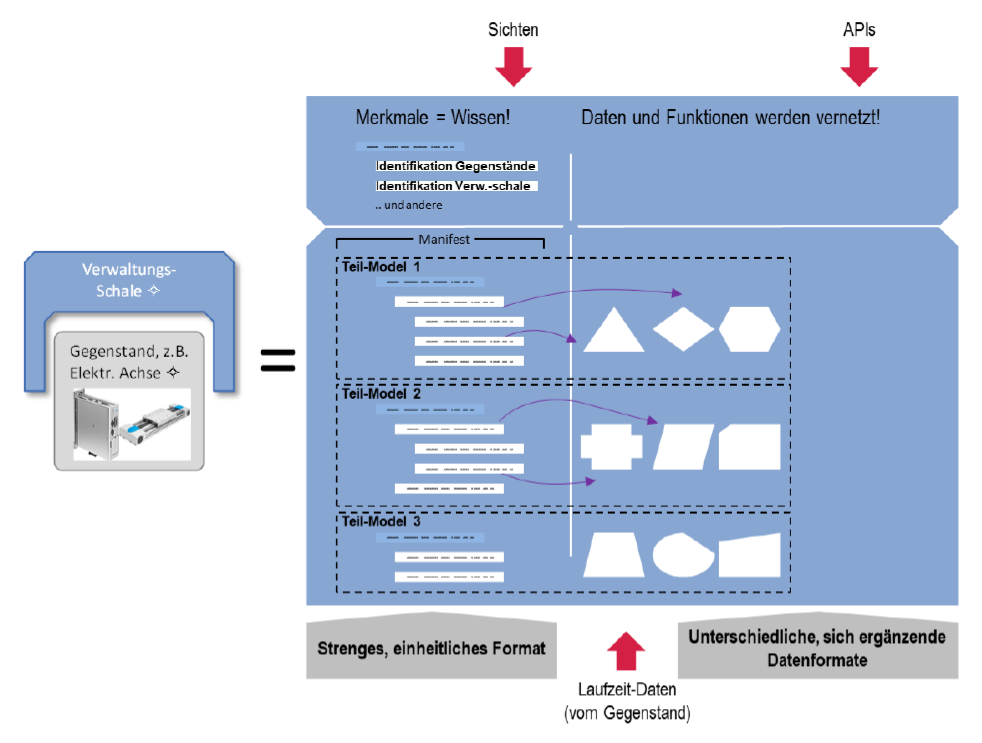
\includegraphics[width=1.1\linewidth]{Struktur_Verwaltungsschale.png}
  \caption[Struktur der Verwaltungsschale]{Struktur der Verwaltungsschale}
  \label{verwaltungsschale}
\end{figure}

\newpage


